% RLC-Parallelschwingkries - Spannungskurve |U| von w/w0 mit Q=1,2,3,4,1000 bei Stromquelle I=Iq
\def\G{10e-3}%  10 mS % variabel
\def\L{10e-3}%  10 mH
\def\C{10e-6}%  10 uF
\def\Bk{31.623}% Bk = sqrt(C/L) = 31.623 mS
\def\Iq{10}     % 10 mA
% w0 = 1/sqrt(LC) = 3162.278 Hz
% Güte Q = Bk/G -> G = Bk/Q
\def\Bk{31.623}
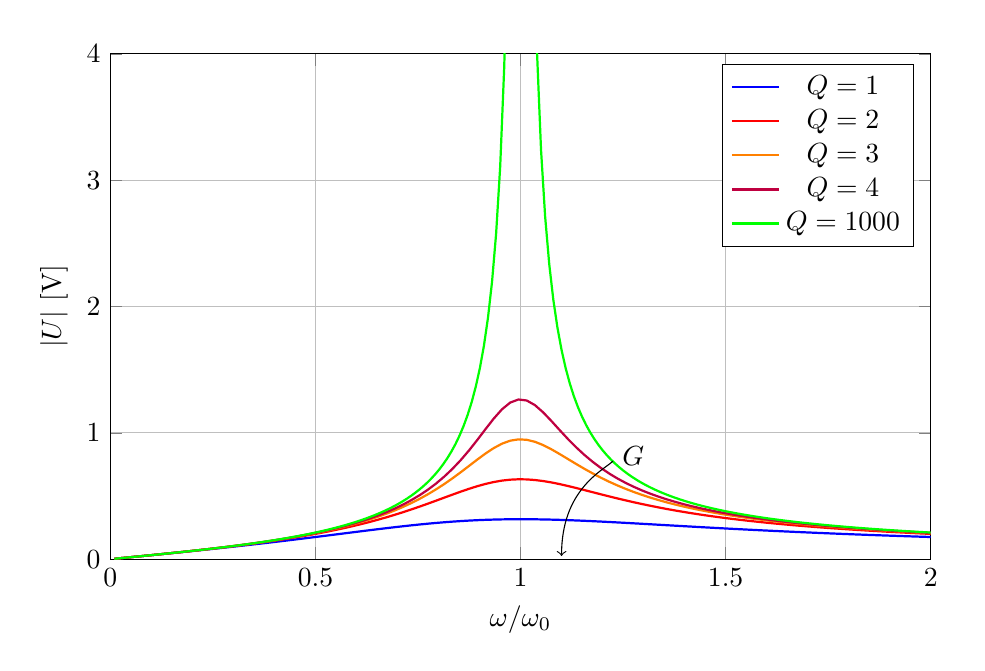
\begin{tikzpicture}[x=1cm,y=1cm]
    \draw[draw=none] (-1.05,-1) rectangle (10.75,6.75); % boundbox (not matching width and height, don't know why)
    \begin{axis}[
        xlabel={$\omega/\omega_0$},
        ylabel={$|U|\ [\mathrm{V}]$},
        xmin=0, xmax=2,
        ymin=0, ymax=4,
        width=12cm,
        height=8cm,
        samples=100,
        grid=both,
        xtick={0, 0.5, 1, 1.5, 2, 2.5, 3},
    ]
    % Y/Bk = G + jBk*(w/w0 - w0/w)
    % |Y|/Bk = sqrt( (1/Q)^2 + (w/w0 - w0/w)^2 )
    % |U| = Iq / |Y| 
    % |U| = Uk * 1/sqrt( (1/Q)^2 + (w/w0 - w0/w)^2 )    # fikt. Referenzspannung    Uk = Iq/Bk
    % |U| = U0 * 1/sqrt( 1 + Q^2 * (w/w0 - w0/w)^2 )    # alt. mit Maximalspannung  U0 = Iq/G
    \addplot[domain=0.01:2.00, thick, color=blue]   {\Iq/\Bk * 1/(sqrt((1/1)^2+(x-1/x)^2))   }; % Güte 1 G=31.62
    \addplot[domain=0.01:2.00, thick, color=red]    {\Iq/\Bk * 1/(sqrt((1/2)^2+(x-1/x)^2))   }; % Güte 2 G=15.81
    \addplot[domain=0.01:2.00, thick, color=orange] {\Iq/\Bk * 1/(sqrt((1/3)^2+(x-1/x)^2))   }; % Güte 3 G=10.54
    \addplot[domain=0.01:2.00, thick, color=purple] {\Iq/\Bk * 1/(sqrt((1/4)^2+(x-1/x)^2))   }; % Güte 4 G=7.91
    \addplot[domain=0.01:0.99, thick, color=green]  {\Iq/\Bk * 1/(sqrt((1/1000)^2+(x-1/x)^2))}; % Güte 1000 G=0.032
    \addplot[domain=1.01:2.00, thick, color=green]  {\Iq/\Bk * 1/(sqrt((1/1000)^2+(x-1/x)^2))}; % Güte 1000 G=0.032
    \addlegendentry{$Q=1$}
    \addlegendentry{$Q=2$}
    \addlegendentry{$Q=3$}
    \addlegendentry{$Q=4$}
    \addlegendentry{$Q=1000$}
    
    % G Steigend 
    \draw [<-](axis cs:1.1,0.025) .. controls (axis cs:1.1, 0.55) and (axis cs:1.2,0.7) .. (axis cs:1.225,0.775); % ca. normale
    \draw(axis cs:1.275, 0.8125)node{$G$};

    \end{axis}
\end{tikzpicture}